\subsection{A recording-level model}\label{a-recording-level-model}

The unit of analysis is the recording, not the window. Write the
transformed recording feature as

\[X_r = A x_r^{(0)} + b \in \mathbb R^p,\qquad Z_r\in\{1,\dots,K\},\]

and define the environment-specific mean, the mixing weight, and the
smallest center separation by

\[\mu_e = E[X\mid Z=e],\qquad \pi_e=P(Z=e),\qquad
\Delta=\min_{e\ne f}\|\mu_e-\mu_f\|.\]

The population K-means risk and its optimum are

\begin{equation}\label{eq:risk}
R(c)=E\!\left[\min_k\|X-c_k\|^2\right],\qquad R^\star=\inf_c R(c).
\end{equation}

\begin{definition}[center space, tie-breaking, and the misclassification rate]\label{def:err}
A center configuration is an ordered $K$-tuple $c=(c_1,\dots,c_K)$ in $(\mathbb R^p)^K$, and configurations that differ only by the relabeling action of the symmetric group $S_K$ are identified in the quotient $(\mathbb R^p)^K/S_K$. The bounded center domain is $\mathcal C_B=(\overline{\mathcal B_p(B)})^K/S_K$. For a configuration $c$, the nearest-center rule is $g_c(x)=\arg\min_k\|x-c_k\|^2$, with ties broken by a fixed measurable rule so that $g_c$ is defined at every point. The misclassification rate is
$$\mathrm{Err}(c,Z)=\min_{\tau\in S_K}P\{g_c(X)\ne\tau(Z)\},$$
which is invariant to label permutation and takes values in $[0,1]$.
\end{definition}

The model is conditional on the feature the pipeline builds,
\(X_r=A[\frac1{W_r}\sum_w\operatorname{vech}\{\log(\widehat\Sigma_{rw})\}]+b\).
Window-level dependence enters the residual, and the recording variance
is governed by the effective window count \(T_{\rm eff}\), not the
nominal \(W_r\). The systematic
Ledoit--Wolf~\cite{ledoit2004} and matrix-log bias
shifts the center, with \(E[\mu_{e,T}]-\mu_e=O(T_{\rm eff}^{-1})\),
while the random fluctuation is noise. The finite-sample theorem treats
\((A,b)\) as a pre-given, deterministic transformation. A StandardScaler
fitted on the data stays random even when frozen afterwards, so it does
not meet this condition. A full-pool scaler belongs to the transductive
variant, and a scaler fitted on the training subset is treated as an
empirical variant.

\subsection{Assumptions}\label{assumptions}

We work with a location model \(X=\mu_Z+\xi_Z\), where
\(E[\xi_e\mid Z=e]=0\).

The assumptions separate into two layers. The first layer,
Assumptions~\ref{a:weights}--\ref{a:sep} together with
the population alignment in Assumption~\ref{a:align},
gives zero-error recovery of the population global minimizer. The second
layer, the closed level sets in
Assumption~\ref{a:closed} and the quadratic growth in
Assumption~\ref{a:growth}, is used only for the positive
risk gap and the quantitative risk-transfer statements; neither is
needed for the zero-error result.

\begin{assumption}[weights]\label{a:weights}
$\pi_e\ge\pi_{\min}>0$ for every $e$.
\end{assumption}

\begin{assumption}[concentration, hard ball]\label{a:conc}
$\|\xi_e\|\le\rho$ almost surely.
\end{assumption}

\begin{assumption}[separation]\label{a:sep}
$\Delta>4\rho$.
\end{assumption}

The hard-ball and separation assumptions define an idealized benchmark,
not the empirical setting of this paper. They are geometric premises
used to state the conditional transfer cleanly, and they are not
satisfied by Gaussian or sub-Gaussian residuals, whose support is
unbounded, or by the EEG covariance features. The experiments do not
claim otherwise. The next section lifts them to unbounded sub-Gaussian
tails through a high-probability argument.

For a point from environment \(e\), its distance to its own center is at
most \(\rho\), while \(\|X-\mu_f\|\ge\Delta-\rho>3\rho>\|X-\mu_e\|\) for
\(f\ne e\). This gives the next lemma.

\begin{lemma}[the true-center classifier is correct]\label{lem:truecenter}
Under Assumptions~\ref{a:weights}--\ref{a:sep}, the nearest-center classifier at the true centers satisfies $g_\mu(X)=Z$ almost surely.
\end{lemma}

The lemma says only that the true centers classify correctly; it does
not say they solve the population K-means problem.

\begin{assumption}[population K-means alignment]\label{a:align}
For fixed $K$ and a pre-given transformation, every global minimizer of the population K-means risk assigns exactly one center to each environment:
$$\mathcal C^\star=\{c:R(c)=R^\star\}=\{(\mu_1,\dots,\mu_K)\text{ up to label permutation}\}.$$
The set $\mathcal C^\star$ is the optimizer set within the bounded domain $\mathcal C_B$, not an unconstrained full-space minimizer; the radius $B$ is taken large enough that every environment mean lies in $\overline{\mathcal B_p(B)}$.
\end{assumption}

This is a direct condition on the geometry of the population objective,
not a consequence of any split or merge calculation, and it is stronger
than pairwise mean separation. It identifies the entire global optimizer
set, not merely the correctness of the nearest-mean classifier.

\begin{lemma}[boundary-tube vanishing on a non-degenerate center domain]\label{lem:closed}
In the bounded frame $\|X\|\le B$ with the law of $X$ absolutely continuous, on the non-degenerate domain $\mathcal C_{B,d_{\min}}$ where distinct centers stay at least $d_{\min}$ apart, $\mathrm{Err}(c,Z)$ is continuous and every level set is closed.
\end{lemma}

\begin{assumption}[closed level sets]\label{a:closed}
The misclassification function $\mathrm{Err}(c,Z)$ is upper semicontinuous on the center domain; equivalently, every level set $\mathcal C_q=\{c:\mathrm{Err}(c,Z)\ge q\}$ is closed. On the non-degenerate domain this follows from Lemma~\ref{lem:closed}; on the full domain, including coincident centers, it is retained as an explicit assumption.
\end{assumption}

The lemma does not cover coincident centers, where an arbitrarily small
perturbation can place the new bisector through a region of positive
probability; the one-dimensional counterexample is given in Appendix
A.5.

\begin{assumption}[quadratic growth]\label{a:growth}
$R(c)-R^\star\ge\kappa_0\,d(c,\mathcal C^\star)^2$, where $d(c,\mathcal C^\star)=\min_{\pi\in S_K}\big(\sum_k\|c_k-\mu_{\pi(k)}\|^2\big)^{1/2}$ is the distance on the quotient $\mathcal C_B$, minimized over label permutations. The constant $\kappa_0$ is distinct from the fourth-order cumulant $\kappa_{ijkl}$ used in Chapter 4.
\end{assumption}

This is an independent strong assumption. The margin condition does not
imply it, and the quantitative bound it supports is local. The split and
merge quantities used in the diagnostics are reported as descriptive
only; they do not establish population optimality, and the local
exchange argument built on them has been withdrawn.

\subsection{The conditional compatibility
theorem}\label{the-conditional-compatibility-theorem}

The recording-level guarantee follows a fixed route: population
alignment identifies the optimal centers, a positive risk gap converts
excess risk into a label-error bound, and uniform control of the
empirical risk turns that into a finite-sample statement. The theorem is
conditional on the population K-means alignment above, which fixes the
whole global optimizer set rather than only the nearest-mean decision
rule; it is not an identification result derived from the generative
model.

\begin{theorem}[conditional population recovery under K-means alignment]\label{thm:A}
Suppose Assumptions~\ref{a:weights}--\ref{a:sep} and Assumption~\ref{a:align} hold. Then for some permutation $\pi$,
$$P\{g_{c^\star}(X)\ne\pi(Z)\}=0.$$
\end{theorem}

\emph{Proof sketch.} Assumption~\ref{a:align} identifies
the optimal centers as a permutation of the means, which
Lemma~\ref{lem:truecenter} makes error-free. The full
proof is in Appendix A.3.

The recovery comes from the alignment that is assumed, not from a
lower-level generative argument. The Conditional Compatibility Theorem
states that K-means compatibility implies risk-gap recovery; it is not a
generative bridge from recording separation to partition recovery.

For a target misclassification level \(q\), set

\begin{equation}\label{eq:margin}
\mathcal C_q=\{c:\mathrm{Err}(c,Z)\ge q\},\qquad
\psi(q)=\inf_{c\in\mathcal C_q}\{R(c)-R^\star\}.
\end{equation}

\begin{lemma}[compact center domain and continuity of the risk]\label{lem:compact}
In the bounded-feature frame $\|X\|\le B$, the center space $\mathcal C_B$ is compact, the population risk $R$ is continuous on it, and an optimizer can be taken inside $\mathcal C_B$.
\end{lemma}

\begin{theorem}[positive risk gap]\label{thm:B}
Under the assumptions of Theorem~\ref{thm:A} together with Assumption~\ref{a:closed}, for every $q>0$ with $\mathcal C_q\ne\varnothing$,
\begin{equation}\label{eq:compatibility}
\psi(q)>0.
\end{equation}
\end{theorem}

\emph{Proof sketch.} The optimal set has error zero, so the closed level
set \(\mathcal C_q\) excludes it. Compactness and continuity then force
the infimum of \(R-R^\star\) to be attained and strictly positive. The
full proof is in Appendix A.3.

A quantitative form is available only locally. Let the margin obey
\(P(X\in\mathcal M_t)\le C_{\rm margin}t^\beta\), with \(\beta=1\) in
the ordinary case. Inside the local stability region, combining the
margin relation with Assumption~\ref{a:growth} gives

\[\psi(q)\ge\kappa_0\Big(\frac{q}{C_{\rm margin}}\Big)^{2/\beta}\quad\text{for }0<q\le q_0.\]

For \(\beta=1\), \(\psi(q)\ge(\kappa_0/C_{\rm margin}^2)q^2\). The
cutoff \(q_0\) is the largest level at which the local linearization
holds. We claim no global quantitative bound, and neither \(\kappa_0\)
nor \(C_{\rm margin}\) is self-certified.

\subsection{Finite-sample transfer}\label{finite-sample-transfer}

Let \(\widehat R_M\) be the empirical risk on \(M\) independent
recordings, let
\(\varepsilon_M=\sup_{c\in\mathcal C}|\widehat R_M(c)-R(c)|\), and let
\(\delta_{\rm opt}=\widehat R_M(\widehat c)-\widehat R_M^\star\) be the
optimization error. The standard excess-risk decomposition is

\begin{equation}\label{eq:risk-gap}
R(\widehat c)-R^\star\le 2\varepsilon_M+\delta_{\rm opt}.
\end{equation}

\begin{lemma}[risk transfer]\label{lem:transfer}
Fix $q>0$ with the level set $\mathcal C_q$ closed so that $\psi(q)$ is well defined. For any configuration $\widehat c$,
$$R(\widehat c)-R^\star<\psi(q)\quad\Longrightarrow\quad \mathrm{Err}(\widehat c,Z)<q.$$
Combined with the excess-risk decomposition, $2\varepsilon_M+\delta_{\rm opt}<\psi(q)$ implies $\mathrm{Err}(\widehat c,Z)<q$.
\end{lemma}

The implication is conditional: it does not assume alignment and does
not assert that \(\psi(q)\) is positive. For bounded features, the
uniform deviation admits an explicit grid bound. An \(\eta\)-net of the
stacked center domain has size \(N_\eta\le(1+2\sqrt K B/\eta)^{Kp}\),
and the cell function is \(4B\)-Lipschitz in the product center norm. A
Hoeffding bound and a union over the net give, with probability at least
\(1-\alpha\),

\[\varepsilon_M\le h(M,\eta),\qquad
h(M,\eta)=\sqrt{\frac{8B^4\log(2N_\eta/\alpha)}{M}}+8B\eta.\]

The covering, Lipschitz, and Hoeffding derivation is in Appendix A.4.

\begin{corollary}[nontrivial finite-sample recovery]\label{cor:finite}
Suppose every assumption of Theorem~\ref{thm:B} holds and choose $q$ with $\psi(q)>0$. For a global empirical minimizer, $\delta_{\rm opt}=0$, and if
$$2h(M,\eta)<\psi(q),$$
then with probability at least $1-\alpha$, $\mathrm{Err}(\widehat c,Z)<q$. For a finite-initialization Lloyd solution the same conclusion holds with probability at least $1-\alpha$ under $2h(M,\eta)+\delta_{\rm opt}<\psi(q)$.
\end{corollary}

\emph{Proof sketch.} On the event \(\varepsilon_M\le h(M,\eta)\), the
excess-risk decomposition gives excess risk below \(\psi(q)\), and the
risk-transfer lemma then yields \(\mathrm{Err}(\widehat c,Z)<q\). The
positivity \(\psi(q)>0\) is the content of
Theorem~\ref{thm:B}; without it the bound is the empty
conditional.

\subsubsection{High-probability sub-Gaussian
truncation}\label{high-probability-sub-gaussian-truncation}

The hard-ball radius is a deterministic support bound. A sub-Gaussian
tail replaces it with a radius that holds with a chosen probability,
with no bounded-support requirement.

\begin{assumption}[sub-Gaussian residuals]\label{a:sg}
There is a constant $\sigma\ge 0$ such that, for every environment $e$ and every $v\in\mathbb R^p$, $\|\langle v,\xi_e\rangle\|_{\psi_2}\le \sigma\|v\|$. Here $\|Y\|_{\psi_2}=\inf\{t>0:E[\exp(Y^2/t^2)]\le 2\}$ is the sub-Gaussian Orlicz norm.
\end{assumption}

For a sub-Gaussian vector in \(\mathbb R^p\), there are universal
constants \(C_1,c_2>0\) such that
\[P\big(\|\xi_e\|>C_1\sigma(\sqrt p+t)\big)\le 2\exp(-c_2t^2/\sigma^2).\]
For \(\delta\in(0,1)\), define the high-probability radius
\[\rho_\delta=C\sigma\sqrt{p+\log(K/\delta)},\] where \(C\) is
universal. A union bound over the \(K\) environments gives
\[P\big(\max_e\|\xi_e\|>\rho_\delta\big)\le\delta.\]

\begin{proposition}[conditional lift under truncation]\label{prop:trunc}
Let $E_\delta=\{\max_e\|\xi_e\|\le\rho_\delta\}$. On $E_\delta$, which has probability at least $1-\delta$, the hard-ball assumptions hold with $\rho$ replaced by $\rho_\delta$. If $\Delta>4\rho_\delta$ and the population alignment in Assumption~\ref{a:align} holds on the truncated population, the zero-error classification, the conditional recovery of Theorem~\ref{thm:A}, and the finite-sample Corollary~\ref{cor:finite} carry over, conditioned on $E_\delta$, with $\rho_\delta$ in place of $\rho$.
\end{proposition}

For a finite sample of \(M\) independent recordings, the union bound is
over the \(M\) observations and the radius becomes
\(\rho_{\delta,M}=C\sigma\sqrt{p+\log(KM/\delta)}\), with the same
probability and the same conditional conclusion.

Three qualifications are part of the statement. First, truncation
relaxes the support condition only; the population alignment remains an
explicit premise, and the proposition does not derive it. Second, the
radius and the required separation grow as \(\sqrt{\log(1/\delta)}\), so
higher confidence demands a larger separation, the cost of unbounded
support. Third, outside \(E_\delta\), an event of probability at most
\(\delta\), the hard-ball conclusion is not asserted; with a bounded
loss the unconditional statement adds a term of order \(\delta\).

\subsection{The DELVE procedure and operational
variants}\label{the-delve-procedure-and-operational-variants}

The estimand and the guarantee are operationalized by one procedure,
listed in Algorithm~\ref{alg:delve}. The bracketed tags
separate standard components from this paper's estimand and guarantee.

\begin{algorithm}[H]
\centering
\small
\renewcommand{\arraystretch}{1.15}
\begin{tabular}{@{}r >{\raggedright\arraybackslash}p{0.78\columnwidth}@{}}
\textbf{Input} & recordings $\{R_1,\dots,R_M\}$, grid $\mathcal K=\{2,\dots,6\}$, level $\alpha$\\
\textbf{Output} & $\hat K$, hard labels $\hat\ell_r$, soft posteriors $\eta_{rk}$, stability, bootstrap, sensitivity\\
\textbf{Stage 0} & [standard] homogenize: shared channels, common-average reference, band-pass with notch, resample, four-second windows\\
\textbf{Stage 1} & [standard] per window $\widehat\Sigma_w=\mathrm{LedoitWolf}$; $x_w=\operatorname{vech}(\log\widehat\Sigma_w)$\\
\textbf{Stage 2} & [this paper's estimand] $x_r=\frac1{W_r}\sum_w x_w$; $X=\mathrm{StandardScaler}$ across recordings\\
\textbf{Stage 3} & [standard] K-means fitting followed by nearest-centroid assignment; BIC, silhouette, and stability score; $\hat K$\\
\textbf{Stage 4} & [theoretical guarantee, not a computed output] the conditional misclassification statement of Corollary~\ref{cor:finite}; its terms are population quantities, and the procedure evaluates no numeric bound\\
\textbf{Stage 5} & [standard] co-assignment and resampling stability\\
\textbf{Stage 6} & [standard] assignment bootstrap and perturbation sensitivity\\
\textbf{Stage 7} & post-hoc interpretation using metadata, not an algorithm output\\
\end{tabular}
\caption{The DELVE procedure for recording-level environment recovery. The standard components (Stages 0--1, 3, 5--6) are not claimed as novel; the contribution lies in the unified recording-level estimand (Stage 2) and the conditional misclassification guarantee (Stage 4). Automatic $K$ selection and the full-pool scaler stay outside the unconditional guarantees.}
\label{alg:delve}
\end{algorithm}

The same staged flow is shown as a diagram in
Figure~\ref{fig:pipeline}.

\begin{figure}[htbp]
\centering
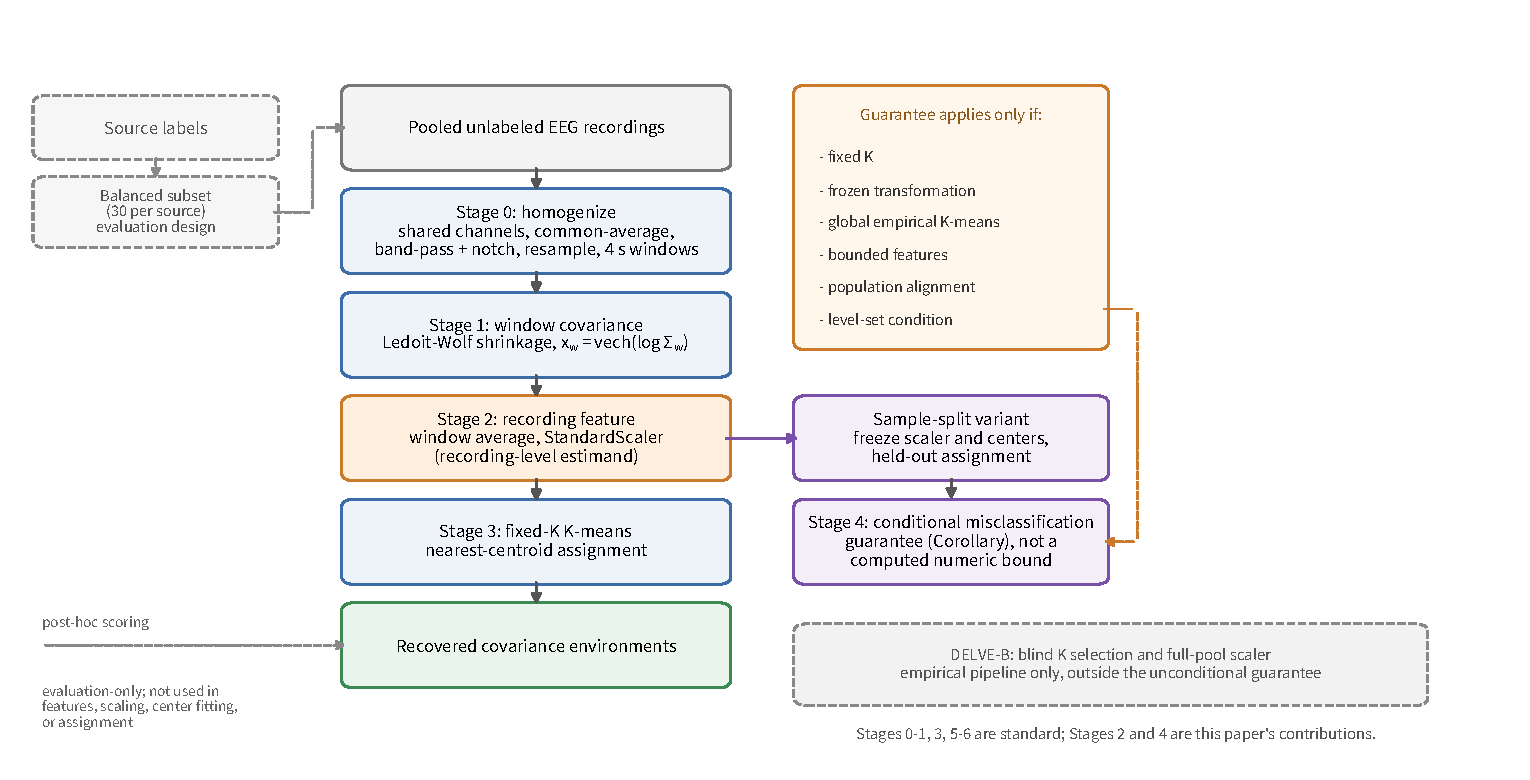
\includegraphics[width=0.74\columnwidth]{fig6_pipeline.pdf}
\caption{Core DELVE processing pipeline and evaluation-only label usage. The staged core runs from pooled unlabeled EEG to recovered covariance environments; the recording-level estimand (Stage 2) is highlighted, and the sample-split branch leads to the Stage 4 conditional misclassification guarantee, a theoretical statement, not a computed numeric bound. The source labels (dashed) are used only to construct the prespecified balanced evaluation subset, thirty recordings per source, and for post-hoc scoring; they are not used to construct features, fit the scaler, select centers, or assign clusters. The remaining stages are standard components.}
\label{fig:pipeline}
\end{figure}

The two-way sample-split fits the scaler and centers on one half and
freezes them for the held-out half. Because the scaler and centers share
the same training data, this is an empirical inductive variant, not the
conditional theorem. A strict three-way split separates the scaler,
center, and evaluation recordings, so the scaler is independent of the
center fit and the held-out assignment; we report it as an inductive
empirical check. The three operational variants, fully compared in
Supplementary Table S6, are DELVE-G, which fixes \(K\) and uses a
pre-given transformation and a global minimizer with zero optimization
error and is covered in full by the risk-gap guarantee; DELVE-L, which
keeps fixed \(K\) but uses finite-initialization Lloyd and carries the
explicit \(\delta_{\rm opt}\); and DELVE-B, the blind pipeline with a
data-dependent scaler and a prespecified selector, which carries no
unconditional guarantee.

Freezing a fitted scaler does not make it pre-given. The guarantee
attaches to the global empirical K-means solution under fixed \(K\), a
pre-given transformation, bounded features, and the alignment and
level-set assumptions. Automatic \(K\) selection, data-dependent
standardization, and finite-initialization Lloyd fall outside it, and
the paper does not establish that the unlabeled EEG satisfies the
conditions. Proving alignment on a structured distribution class through
a capture or exchange argument is left as future work.
